\documentclass[handout]{beamer}

\usepackage{Haust2016glærur}

\title{Stærðfræðimynstur í tölvunarfræði}
\subtitle{Vika 8, fyrri fyrirlestur}

\begin{document}

\begin{frame}
\titlepage
\end{frame}


\section{Inngangur}

\begin{frame}{Í síðasta tíma}
\begin{itemize}
 \item Umraðanir
 \item Samantektir
 \item Tvíliður
\end{itemize}
\end{frame}

\section{Miðmisseriskönnun og viðbrögð}

\begin{frame}{Miðmisseriskönnun}
\begin{center}
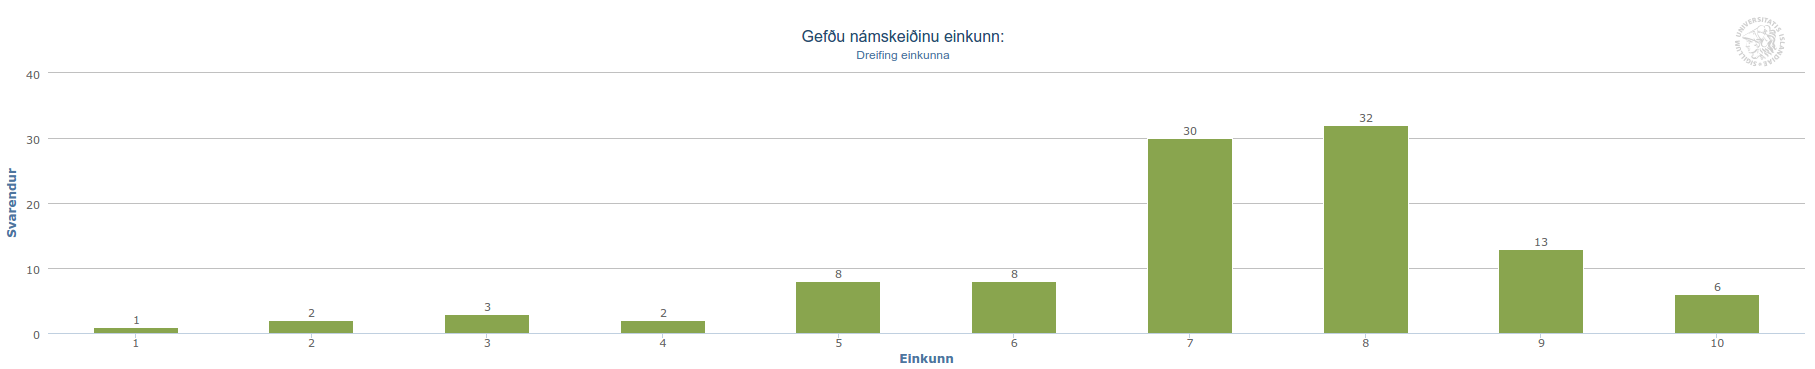
\includegraphics[width=\textwidth]{Dreifing2016}
\end{center}
Meðaleinkunn 7.17 (Meðaleinkunn IVT 7.83).
\end{frame}

\begin{frame}{Almenn ánægja}
\begin{itemize}
 \item Fleiri jákvæðar en neikvæðar athugasemdir bárust um
 \begin{itemize}[<+->]
  \item Persónu kennarans
  \item Glærur
  \item Connect og fyrirlestraræfingafyrirkomulagið
  \item Bókina
  \item Enga skyldumætingu
 \end{itemize}
\end{itemize}
\end{frame}

\begin{frame}{Skiptar skoðanir}
\begin{columns}
\column{0.5\textwidth}
\begin{itemize}
 \item Heimadæmin!
 \begin{itemize}[<+->]
  \item Of erfið
  \item Of létt
  \item Of ruglingsleg
  \item Of ``beint-af-augum''
 \end{itemize}
\end{itemize}
\column{0.5\textwidth}
Þau verða tekin til athugunar
\end{columns}
\end{frame}

\begin{frame}{Má betur fara}
\begin{itemize}
 \item Hljóð í ólagi
 \item Upplestur af glærum \pause
 \begin{itemize}
  \item Hér verður vantað til verka
 \end{itemize}
 \item Fyrirlestrar ekki teknir upp
 \begin{itemize}
  \item Tilraun verður gerð til að taka upp fyrirlestra
  \item Leiði það til minni mætingar verður tilrauninni aflýst
 \end{itemize}
\end{itemize}
\end{frame}

\begin{frame}{Óvinsælt en breytist ekki}
\begin{itemize}
 \item Lausnir á skilaverkefnum munu ekki fara á netið
 \begin{itemize}
  \item Dæmi eru endurnýtt á milli ára
  \item ``Opinberir'' lausnapakkar frá fyrri árum hafa reynst vera svindlseglar
  \item Hægt er að nálgast réttar lausnir í dæmatímum
  \item Þetta sökkar.
 \end{itemize}
 \item Dæmi verða ekki leyst á töflunni í fyrirlestrum
 \begin{itemize}
  \item Kannski á næstu önn
 \end{itemize}
\end{itemize}
\end{frame}

\section{Talning og rakningarvensl}

\begin{frame}{Talning og rakningarvensl}
\begin{itemize}
 \item Sum talningarvandamál eru þess eðlis að erfitt er að leysa þau í einu skrefi
 \item Grípum þá í gamalkunnt tól - rakningarvensl!
 \begin{itemize}
  \item Gætum líka séð fyrir okkur endurkvæmt reiknirit sem ``reiknar út'' fjölda þess sem telja skal
 \end{itemize}
\end{itemize}
\end{frame}

\begin{frame}{Talning á gerlum}
\begin{itemize}[<+->]
 \item Sjáum fyrir okkur að við setjum fimm gerla í skál. Fjöldi gerlanna tvöfaldast á hverjum klukkutíma. Hversu margir verða gerlarnir eftir $n$ klukkutíma?
 \item Látum $n$-ta lið rununnar $\{a_n\}$ tákna fjölda gerla. $n$ Höfum $a_0 = 5$ gerla í upphafi.
 \item Fjöldinn tvöfaldast á hverjum klukkutíma, svo $a_n = 2a_{n-1}$ eftir einn klukkutíma eða meira.
 \item Getum rifjað upp hugmyndir úr kafla 2 til að sjá lokuðu formúluna $a_n = 5\cdot 2^n$
\end{itemize}
\end{frame}

\begin{frame}{Talning á kanínum}
 \begin{itemize}
  \item Ef við setjum nýfætt kanínuungapar á eyðieyju, hversu mörg kanínupör verða á eyjunni eftir $n$ mánuði? Gerum ráð fyrir eftirfarandi:
  \begin{itemize}
   \item Kanínur eru ódrepandi
   \item Kanínur byrja að fjölga sér eftir að þær hafa náð tveggja mánaða aldri
   \item Kanínur sem fjölga sér fjölga sér í hverjum mánuði
   \item Þegar kanínur fjölga sér myndar hvert kanínupar nýtt par
  \end{itemize}
 \end{itemize}
\end{frame}

\begin{frame}{Talning á kanínum}

\begin{center}
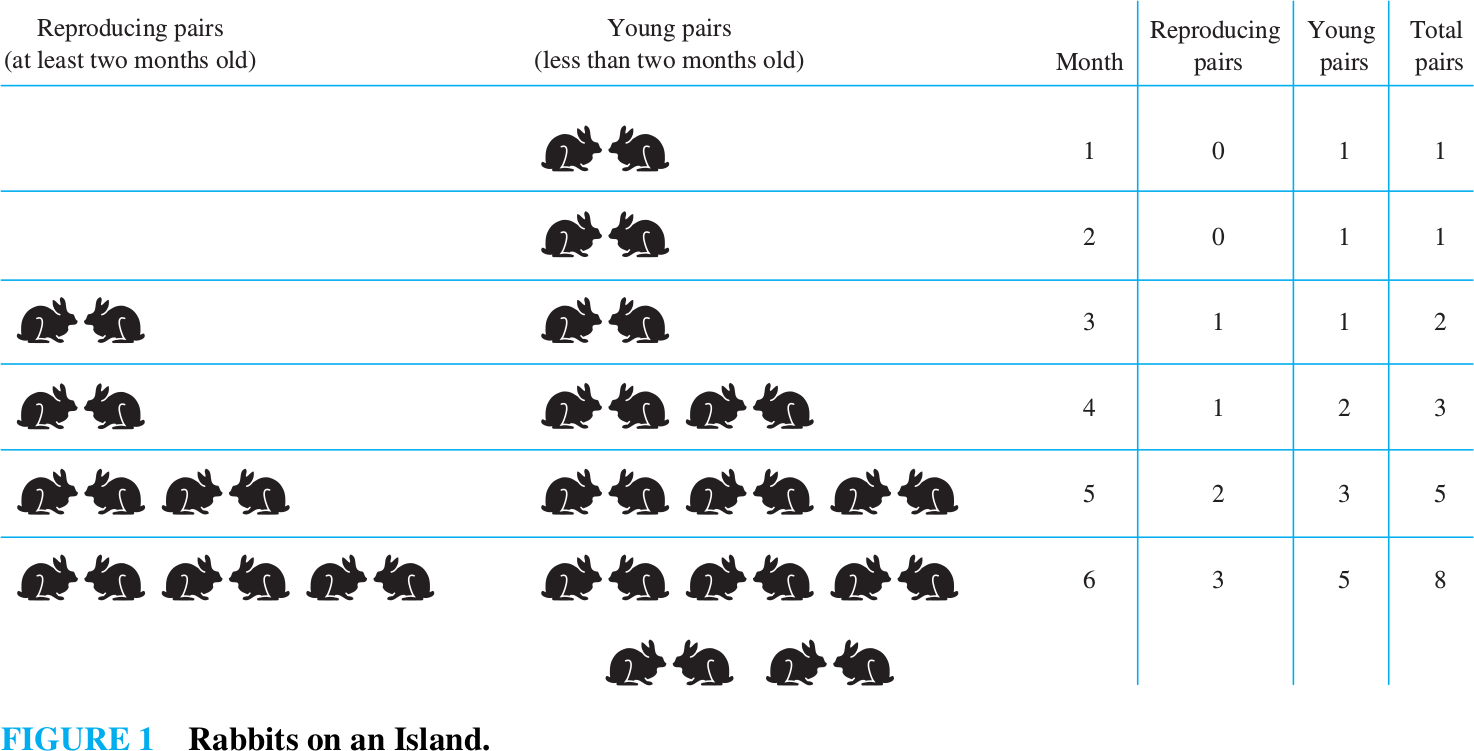
\includegraphics[width=0.8\linewidth]{rabbits}
\end{center}
Fáum út rakningarvenslin $a_1 = 1$, $a_2 = 1$, $a_n = a_{n-1} + a_{n-2}$ fyrir $n \geq 3$.
\end{frame}

\begin{frame}{Turnar Hanoi}
\begin{columns}
\column{0.5\textwidth}
\begin{itemize}
 \item Þrautin ``Turnar Hanoi'' snýst um að færa stafla af skífum á milli pinna
 \begin{itemize}
  \item Viljum færa staflann af pinna 1 yfir á pinna 3
  \item Megum ekki setja skífu ofan á minni skífu
 \end{itemize}
 \item Finnum tölu $H_n$, sem táknar fjölda skífuhreyfinga sem þarf til að leysa þrautina
\end{itemize}
\column{0.5\textwidth}
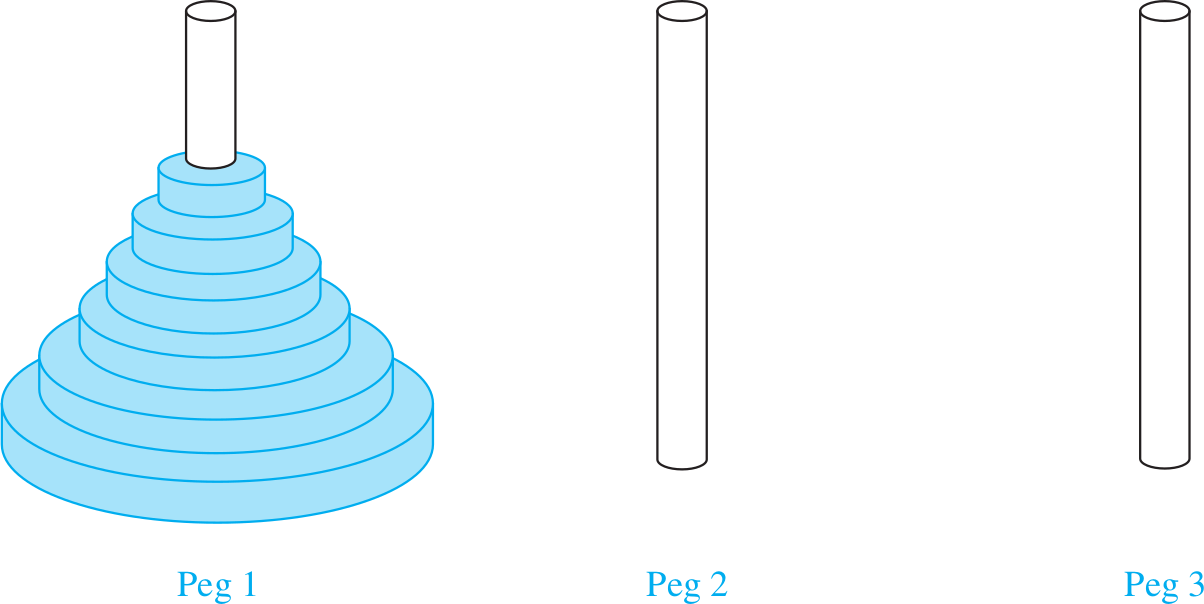
\includegraphics[width=\linewidth]{hanoi}
\end{columns}
\end{frame}

\begin{frame}{Rakningarvensl fyrir turna hanoi}
Finnum rakningarvensl fyrir rununa $\{H_n\}$. \pause

Sjáum að við höfum grunngildið $H_1 = 1$. \pause

Sé hægt að leysa þrautina, þá er hægt að færa fyrstu $n-1$ skífurnar í stafla með $n$ skífum af pinna 1 yfir á pinna 2 í $H_{n-1}$ skrefum. Svo færum við stærstu skífuna yfir á pinna 3. Færum svo $n-1$ skífur af pinna 2 í $H_{n-1}$ skrefum aftur. Hvaða rakningarvensl fáum við? \pause

\[
 H_n = 2H_{n-1} +1
\]
\end{frame}

\section{Kvik bestun}

\begin{frame}{Endurteknir útreikningar}
Ýmis endurkvæm reiknirit láta okkur reikna sömu stærðina oftar en einu sinni. Fibonacci-reikniritið úr kafla 5 er dæmi um slíkt:
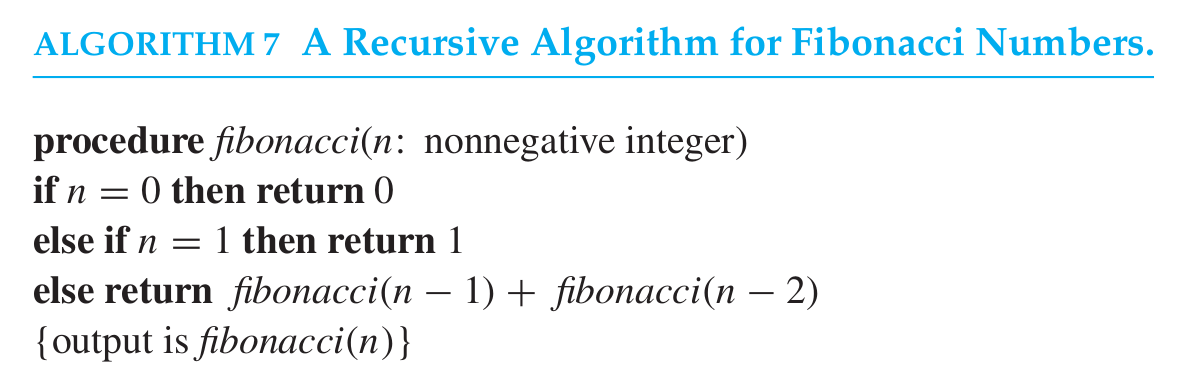
\includegraphics[width=\textwidth]{fibonacci-algorithm}

Endurteknir útreikningar haft mjög slæm áhrif á keyrslutíma forrits.
\end{frame}

\begin{frame}{Endurteknir útreikningar}
\begin{center}
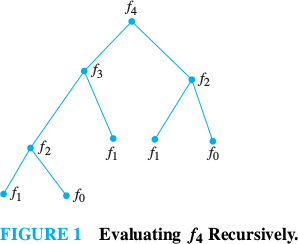
\includegraphics[width=0.6\textwidth]{fibonacci-execution}
\end{center}
\end{frame}

\begin{frame}{Kvik bestun}
\begin{itemize}
 \item Til að forðast endurtekna útreikninga í endurkvæmu reikniriti má notast við kvika bestun (e. \emph{dynamic programming})
 \item Hugmyndin á bak við kvika bestun er brjóta vandamál endurkvæmt niður í smærri vandamál
 \begin{itemize}
  \item Reikna svo út niðurstöðu fyrir smáu tilvikin
  \item Komi smátt tilvik af vandamálinu fyrir aftur, þá má nýta geymdu niðurstöðuna
 \end{itemize}
 \item Kemur oft fyrir í bestunarvandamálum
 \begin{itemize}
  \item Nafnið er annars frekar merkingarlaust
 \end{itemize}
\end{itemize}
\end{frame}

\begin{frame}[fragile]{Skárra fibonacci-reiknirit}
\begin{columns}
\column{0.3\textwidth}
Notum ``utanáliggjandi geymslu'' til að halda utan um gildi sem þegar hafa verið reiknuð. Hér er geymslan vörpun frá $N$ til $N$.
\column{0.7\textwidth}
\begin{verbatim}
reiknirit fib(n: ekki-neikvæð heiltala)
  ef fib(n) er í geymslu:
    skila gildi úr geymslunni
  annars ef n==0:
    skila 1
  annars ef n==1:
    skila 1
  annars
    f := fib(n-1) + fib(n-2)
    setja f í geymslu
    skila f
\end{verbatim}
\end{columns}
\end{frame}

\begin{frame}{Næst}
\begin{itemize}
 \item Lausnir á línulegum rakningarvenslum (8.2)
 \item Deila-og drottna reiknirit (8.3)
\end{itemize}

\end{frame}


\end{document}
